\chapter{System Design}
\label{chap:System}
The system model is developed in three stages. %
The first two stages were developed in MATLAB, %
and consist of a time invariant model %
for simulating the convergence behaviour of %
the LMS algorithms, and a time varying %
model for showing the tracking performance %
in the environment proposed in section %
\ref{sec:MotivatingScenario}. The %
final stage was developed in LabView on the %
National Instruments Universial Software Radio %
Platform (USRP) model 2943R and presents %
a hardware proof of concept for adaptive %
filtering in slowly time varying channels. %
This section will be dedicated to developing %
the system models. Chapter \ref{chap:Results} %
will develop the results that I collected %
and compare them with whats available in the %
literature.

\section{Time Invariant System Model}
\label{sec:TIModel}
\FloatBarrier
\begin{figure}[ht]
	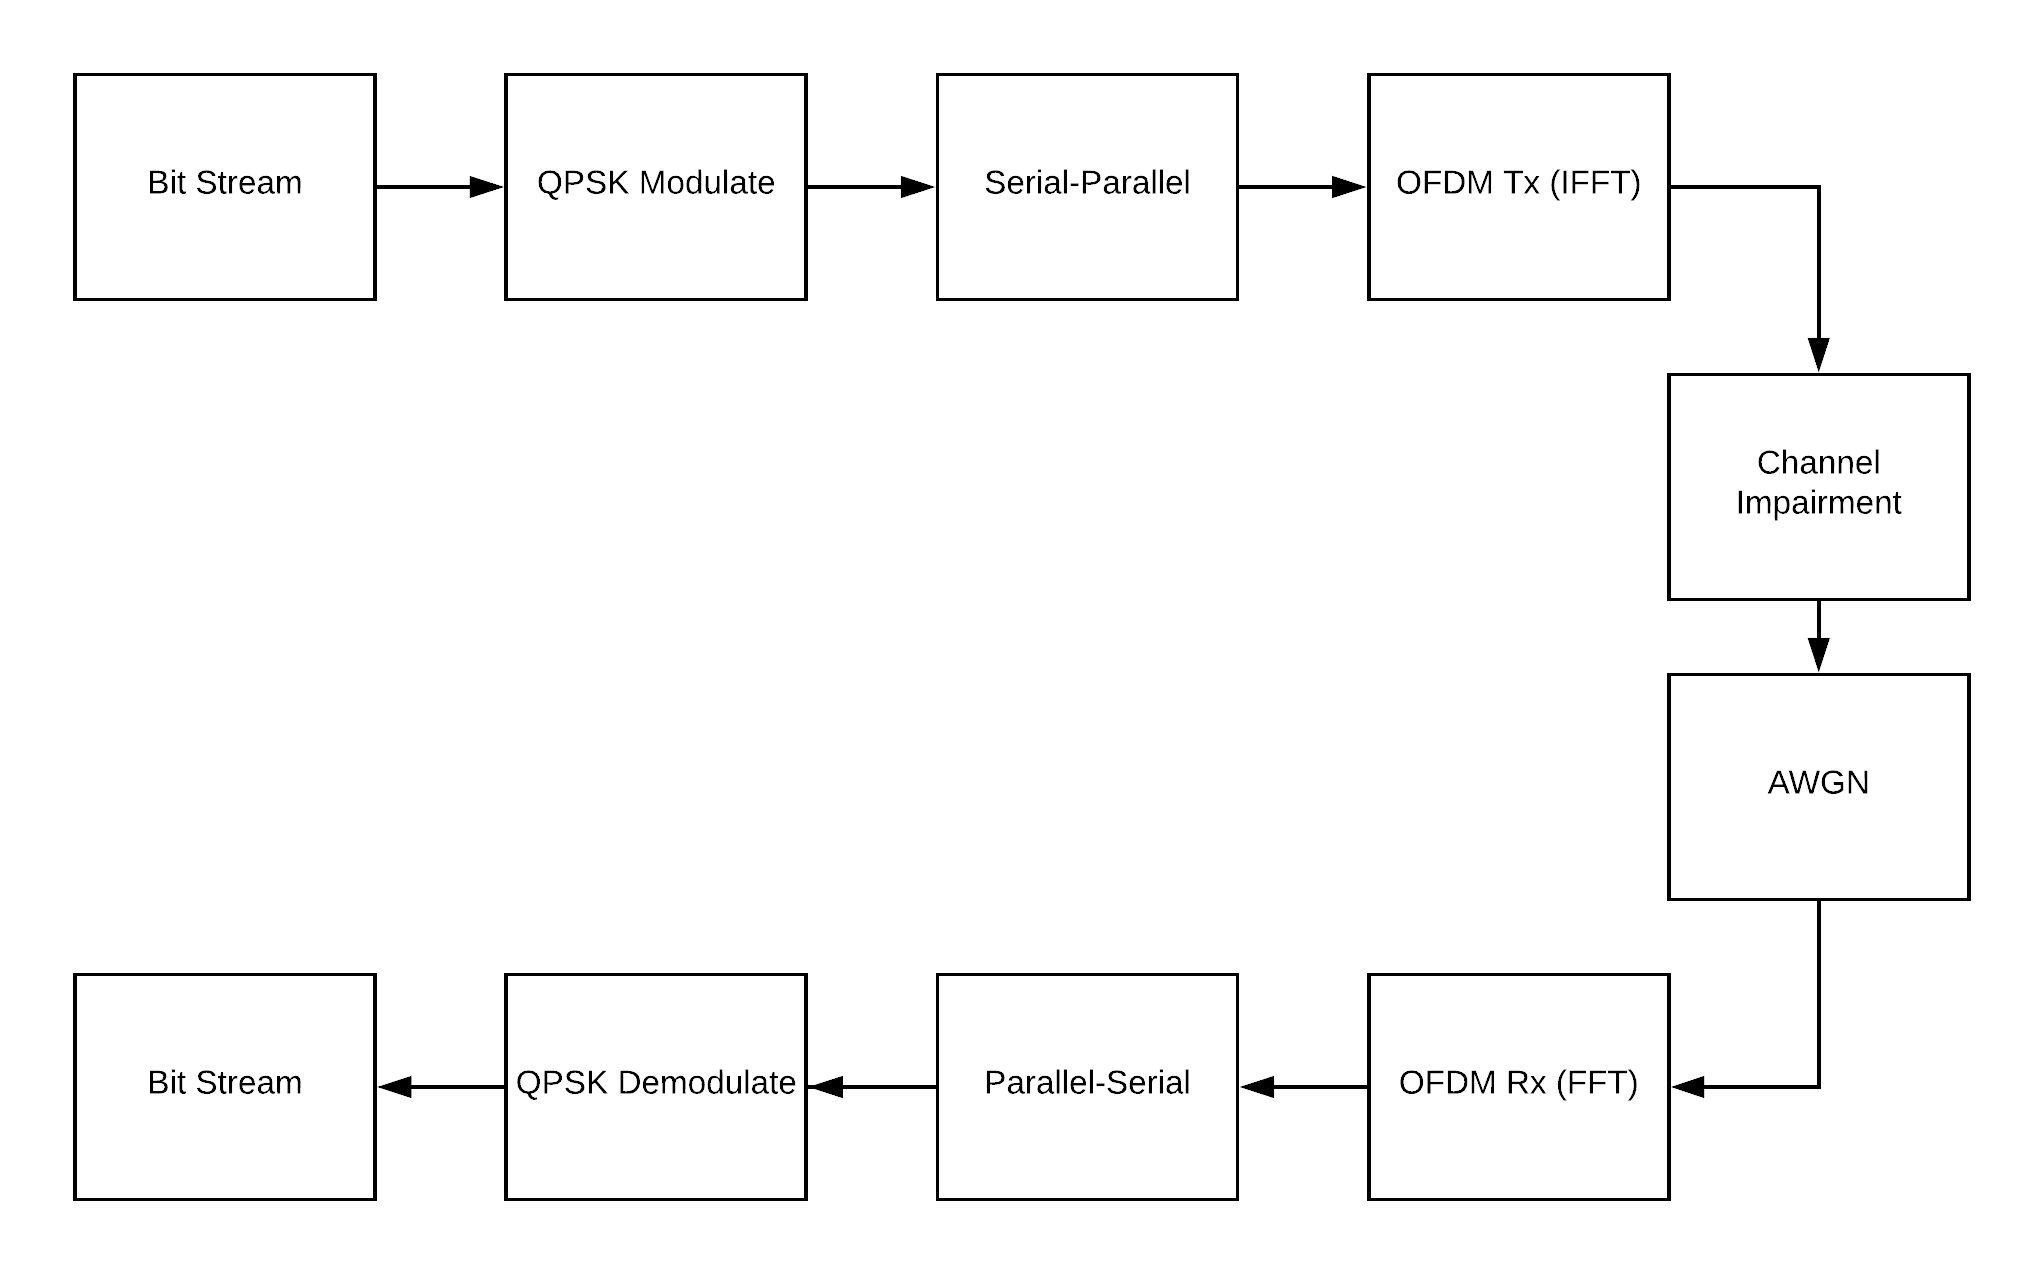
\includegraphics[width=\textwidth]{./%
	Figures/System/SystemModel.png}
	\caption{System Model}
	\label{fig:SysModel}
\end{figure}
Figure \ref{fig:SysModel} depicts the general %
outline of the system model that has been %
developed. This section will focus on %
developing all the components that will %
be common to all the later sections as %
well as section specific components.
\FloatBarrier
The primary aim of the time invariant %
model was to establish the convergence %
of the LMS algorithm with an OFDM %
transmission scheme, equalising in the %
\emph{frequency} domain.
\begin{figure}[ht]
	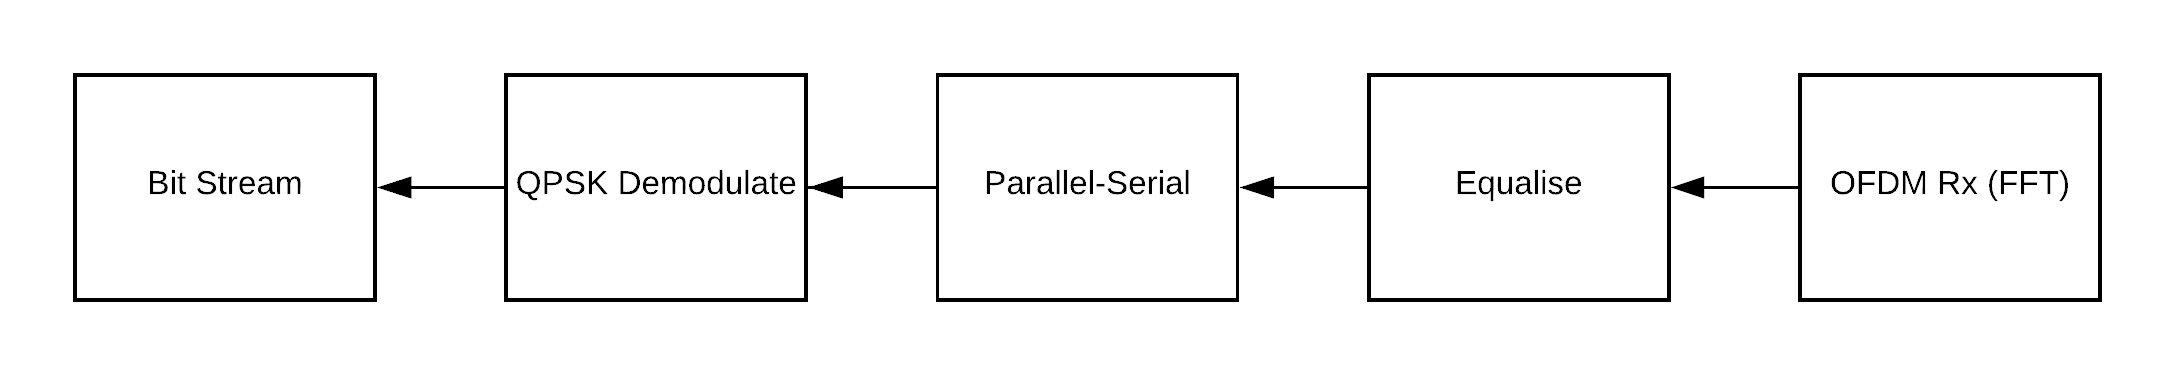
\includegraphics[width=\textwidth]{./%
	Figures/System/RxEqualisation.png}
	\caption{Added equalisation step}
	\label{fig:RxEqualiser}
\end{figure}
Figure \ref{fig:RxEqualiser} illustrates %
the location of the equaliser in this model, %
immediately after the FFT and before the %
parallel to serial step. By designing %
the OFDM subcarrier bandwidth to be %
significantly less than the coherence %
bandwidth of the fading channel a simple %
version of the LMS filter with only one %
filter coefficient can be assigned to %
each subcarrier for equalisation as %
illustrated in figure \ref{fig:Frequency%
LMS}
\FloatBarrier
\begin{figure}[ht]
	\centering
	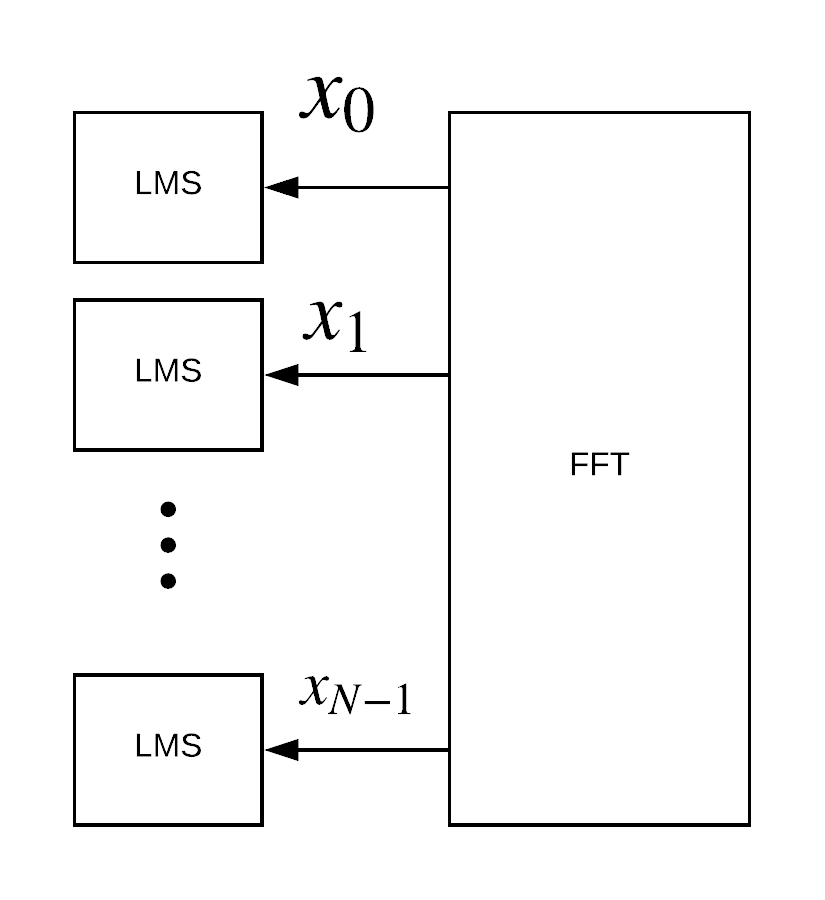
\includegraphics[width=0.5\textwidth]{./%
	Figures/System/FrequencyDomainLMS.png}
	\caption{Single Tap LMS on each Sub%
	carrier}
	\label{fig:FrequencyLMS}
\end{figure}
\FloatBarrier
\subsection{Bit Stream}
The bit stream needs to be selected to model %
a believable source of data. It can be shown %
that without further information, data %
in digital communications systems can be %
modeled as a Bernoulli distribution. %TODO: Cite this
My model simulates this using MATLAB's in-built %
\texttt{randi} function which generates %
a random vector $\bold{X}$ where each %
random variable $X$ can take on values from %
a user defined set of integers and is %
uniformly distributed, i.e. where each integer %
has an equally likely chance of occuring. In %
the special case of the Bernoulli distribution %
the set of integers can be defined as $\{0,1\}$.

\subsection{QPSK Modulation and Demodulation}
\FloatBarrier
QPSK or Quadrature Phase Shift Keying is a popular %
modulation scheme. I've chosen to use it primarily %
for its simplicity but also because it contains both
an in-phase and a quadrature component, which are%
the elements required to construct %
Quadrature Amplitude Modulation (QAM) %
which is the current modulation scheme employed %
in 4G systems % TODO: Find a citation for this.
and is likely to be used in 5G schemes.

\begin{figure}[ht]
	\centering
	\includegraphics[width=0.7\textwidth]{./%
	Figures/System/QPSKScatterplotWithA%
	WGN.png}
	\caption{QPSK Constellation, red stars %
	indicate constellation points, blue %
	points are due to noise}
	\label{fig:QPSKConstellation}
\end{figure}

Figure \ref{fig:QPSKConstellation} shows what %
a QPSK constellation looks like and how a %
received signal might appear when AWGN has %
been added to it. To normalise that average %
symbol energy to 1 the constellation points %
are defined at $\{\frac{\sqrt{2}}{2} + \frac{%
\sqrt{2}}{2}i, \frac{\sqrt{2}}{2} - %
\frac{\sqrt{2}}{2}i, -\frac{\sqrt{2}%
}{2} + \frac{\sqrt{2}}{2}i, %
-\frac{\sqrt{2}}{2} - \frac{\sqrt{2}%
}{2}i\}$ such that when the average %
energy is evaluated
\begin{align}
	E\left[E_s\right] = \frac{1}{4} \sum_{k=1}^{4} %
	\lvert E_{s_{k}} \rvert = 1
\end{align}
where $E_{s_{k}}$ is the symbol energy of the the %
$k\text{th}$ element in the symbol set. A QPSK %
modulation scheme has a symbol set of size $4$. %
So is capable of transmitting $log_{2}(4)$ bits %
per symbol. In general a M-QAM modulation scheme %
is able to transmit $log_{2}(M)$ bits per symbol. %
A grey mapping between pairs of bits to the QPSK %
constellation needs to be chosen so that symbol %
errors that are due to the received symbol mapping %
incorrectly to a neighbouring symbol than what was %
desired will introduce only one bit error instead %
of multiple, it can be shown that grey mapping %
minimises the bit error rate caused by %
symbol errors. %TODO: Find a citation for grey mapping

MATLAB's Communications System Toolbox offers %
a system object name \texttt{QPSKModulator} which %
will perform the grey mapping of pairs of bits in a %
bit stream to QPSK constellation points and perform %
the energy normalisation.

Paired with the \texttt{QPSKModulator} MATLAB also %
provides a \texttt{QPSKDemodulator} which performs %
performs maximum likelihood detection and maps %
the received QPSK constellation back to a bit %
stream.

\subsection{OFDM}

OFDM has been covered in some detail in chapter %
\ref{chap:OFDM} so here I'll focus on the simulation %
implementation. MATLAB's communication systems %
toolbox provides an \text{OFDMModulator} which %
takes in an input stream of symbols and performs %
an IFFT followed by an IFFT shift to place the DC %
components in the centre. It also prepends the %
last $\mu$ samples of the output of the IFFT to %
generate a cyclic prefix and allows the use %
of a DC Null, the DC null will be relevant in %
our discussion on thhe USRP model.

\subsection{AWGN}

The power of additive white gaussian noise $\sigma_n^{2}$ %
was defined relative to the transmit signal power, through %
the following evaluation

\texttt{%
powerdB = 10*log10(var(OFDM\_Symbol));\\%
snr = EbNo + 10*log10(BitsPerSymbol);\\%
noiseVar = 10\textasciicircum(0.1*(powerdB-snr));}

here \texttt{var(OFDM\_Symbol)} is being evaluated %
as 
\begin{align}
	\frac{1}{N} %
	\sum_{n=0}^{N-1} \lvert\lvert \texttt{OFDM\_Symbol}%
	(n) \rvert\rvert^{2}
\end{align}

Where $N$ is the length of the FFT. \texttt{EbNo} is a %
variable which defines the normalised bit energy %
to noise power spectral density and is % TODO: Cite EbNo
expressed as
\begin{align}
	\frac{E_b}{N_0} = \frac{S}{R_b} \div 
	\frac{\sigma_n^{2}}{B}
\end{align}
where $S$ is the average received signal power, %
$R_b$ is the bit rate, $\sigma_n^{2}$ is the %
total additive white gaussian noise power and %
$B$ is the total signal bandwidth. The relation %
between $SNR$ and $E_b/N_0$ is as follows
\begin{align}
	\frac{S}{\sigma_n^{2}} = \frac{E_b}{N_0}
	\frac{R_b}{B}
\end{align}
A modulation scheme such as QPSK doubles the bit %
rate relative to a binary scheme such as on off %
keying or binary phase shift keying (BPSK), so %
SNR needs to be multipled by $2$ for the different %
schemes to experience the same normalised %
signal to noise ratio. In log units multiplication %
is evaluated as addition as can be seen above.

MATLAB's Commmunications System Toolbox system object %
\\\texttt{comm.AWGNChannel} takes an input stream of %
symbols and generates complex gaussian noise with %
zero mean and defined variance. This noise is then %
summed with the samples in the stream to make a noisy %
received signal. In the case of the system model shown in %
figure \ref{fig:SysModel}, the power of the complex %
additive white gaussian noise calculated based on the transmit %
power before channel impairments. This is because the Rayleigh %
fading channel impairment does not affect all subbands equally as %
it is a frequency selective effect, so setting the noise power based %
on the post channel impairment signal would disproportinately affect %
the subcarriers that are experiencing deep fades.

\subsection{Channel Impairment}
\label{sec:TIChannelImpairment}
The channel impairment designed for the time invariant model %
will be different to the channel impairment designed for the time varying model. %
Here the channel impairment will be chosen as a random complex gaussian that %
defines the fading in the frequency domain. For the purpose of testing the convergence %
of the LMS algorithm, a flat fading scenario is introduced where each subcarrier %
is multiplied by the same coefficient $w$ as illustrated in figure \ref{fig:TIChannel}.
\begin{figure}[ht]
	\includegraphics[width=\textwidth]{./Figures/System/%
	ChannelTimeInvariant.png}
	\caption{Time Invariant Flat Fading Channel Model}
	\label{fig:TIChannel}
\end{figure}
By introducing AWGN to the system after channel impairment and then %
applying the LMS individually to each subcarrier in the frequency domain, %
ensemble averages can be taken for differing channel conditions simply by %
increasing the number of subcarriers. A subcarrier count of $1024$ was %
chosen to generate the time invariant results discussed in the next chapter. %

\subsection{Equalisation}

As illustrated in figure \ref{fig:FrequencyLMS}, a frequency domain %
LMS scheme was made with a single tap variant of the LMS algorithm on %
each subcarrier. As discussed in previous chapters, this can be done %
because the subcarrier bandwidths have been designed to be significantly %
narrower than the coherence bandwidth, so can be approximated with a %
single filter coefficient. This approximation has been made explicit in this %
time invariant model as described in section \ref{sec:TIChannelImpairment}. %

The single tap LMS approximation follows closely from the development of the %
LMS filter in section \ref{sec:LMS}, in particular we take equation \ref{eq:SimplifiedLMSUpdate} %
and replace the vector of coefficients $\hat{\bold{w}}(n+1)$ and $\hat{\bold{w}}(n)$ with scalar %
versions, and the vector of filter inputs $\bold{u}(n)$ with a scalar input. Giving the %
new expression
\begin{align}
	\hat{w}(n+1) = \hat{w}(n) + \mu u(n) e^{*}(n)
	\label{eq:ScalarLMS}
\end{align}
This version of the LMS update is the computationally simplest %
the LMS can be with two multiplications and one addition. %
The constant computational complexity of the designed LMS means %
that the complexity of this filtering scheme grows with the %
the size of the FFT needed to ensure that the subcarrier bandwidth %
is narrower than the coherence frequency of the fading channel, and %
has computational complexity $\mathcal{O}(N log(N))$. This scalar version %
of the LMS filter is substituted into the LMS blocks shown in figure %
\ref{fig:FrequencyLMS} at the receiver.

In a similar fashion the NLMS filter can be developed with a scalar equation %
\begin{align}
	\hat{w}(n+1) = \hat{w}(n) + \frac{\mu}{\lvert u(n) \rvert^{2}} %
	u(n) e^{*}(n)
	\label{eq:ScalarNLMS}
\end{align}
and substitued into the LMS blocks in figure \ref{fig:FrequencyLMS} to %
evaluate the performance of the NLMS filter.

\section{Time Varying System Model}

The time varying system model only contains two key differences to the %
time invariant model. The first is the introduction of the time-varying Rayleigh %
and Rician channel models, these channel models have been simulated using %
the filtered white gaussian noise method. The Rayleigh and Rician fading %
channels introduce design constraints to the model not present in the %
simplified time invariant model examined in the previous section %
regarding subcarrier bandwidth and coherence frequency %
as well as the OFDM symbol time and channel coherence time. The second %
key difference is the introduction of a decision directed scheme for the LMS %
filter to examine its tracking performance after achieving the optimal Wiener solution.

\subsection{Filtered White Gaussian Noise Channel Simulation}

The time varying fading channel can be broken down into three %
steps. The power delay definition needs to be defined, using the %
power delay profile the average powers of each multipath tap can %
be defined. Once this is done the time varying component of the %
fading channel needs to be introduced, the method of choice %
for this simulation will be one of filtered white gaussian noise. %
\subsubsection{The Power Delay Profile}

The power delay profile is critical in scaling the average power %
of each multipath coefficient. In figure \ref{fig:ChannelFilterSimulation} %
an illustration of the simulation mechanism by which a single channel %
coefficient process can be generated, $\sigma_{n}$ represents %
is the scaling factor to ensure that the $n\text{th}$ coefficient %
of the multipath channel $h(\tau_{n};t)$ has average power %
$\sigma_{n}^{2}$. In the simplest form of an uncorrelated %
tap-gain model \cite{Jer00} 
\begin{align}
	E\left[\lvert h(\tau_{n};t) \rvert^{2} \right] = %
	\sigma_{n}^{2} = T^{2}p(nT)
	\label{eq:TapPower}
\end{align}
where $p(nT)$ is the sampled version of a diffuse power %
delay profile where $T$ is the sampling period. Or of a %
discrete multipath channel where the multipath coefficients %
are symbol spaced. For the purpose of my investigation I %
will not consider the case of a discrete multipath channel %
where the multipath channel coefficients are not symbol %
spaced since in general this requires us to filter the power %
delay profile by the measurement bandlimiting filter (i.e., matched filtering) %
and so more information would be needed about the pulse shaping %
used. With symbol spacing an assumption is made that the filters used %
are nyquist in nature and so there are no additional components %
introduced by neighbouring multipath coefficients.

\subsubsection{Filtered White Gaussian Noise}

In chapter \ref{chap:ChannelModeling} the time-varying nature of %
the fading channel was established as being closely related to the %
doppler shift of the signal and the maximum doppler frequency $f_d$. %
The doppler spectrum chosen for simulation is the Jakes spectrum as %
defined in equation \ref{eq:JakesSpectrum} as it is a popular spectrum %
widely used in the literature. %TODO: Cite the literature

The filtered white gaussian noise approach aims to recreate this %
time varying effect by directly filtering the random noise representing %
the scattering with a doppler spectrum in the frequency domain\cite{%
MIMO-OFDM10, Iskander}. 
\begin{figure}[ht]
	\includegraphics[width=\textwidth]{./Figures/System/%
	FilteringProcess.png}
	\caption{Channel Filter Tap Generation}
	\label{fig:ChannelFilterSimulation}
\end{figure}
Figure \ref{fig:ChannelFilterSimulation} illustrates the process used %
to generate each individual coefficient in the discrete multipath channel. %
$z(t)$ is an independent and identically distributed time series where %
at each timestep $t$, $z(t)\sim\mathcal{N}(0,1)$ (is normally distributed %
with mean $0$ and standard deviation $1$), $S(\nu)$ is the Jakes doppler %
spectrum as described in equation \ref{eq:JakesSpectrum} and $\sigma_n$ is %
a scaling factor to ensure the average power of the tap matches that of the %
power delay profile.

MATLAB's Communications System Toolbox provides a system object %
\\\texttt{comm.RayleighChannel}, which implements the filtered %
white gaussian noise method of simulation as described in \cite{Iskander}. %
Rician distributions are implemented slightly differently where the Rician %
taps are further scaled by a deterministic component with a specular to %
scattered power ratio $K$ as described in equation \ref{eq:KFactor}. The %
Rician fading component is scaled by
\begin{align}
	h(\tau;t) = \sigma_n\left[ \frac{z_{k}\left[n\right]}{\sqrt{K + 1}} + 
	\sqrt{\frac{K}{K+1}}\right]
\end{align}
Where $z_{k}$ is the filtered noise output of the doppler filter \cite{Iskander} %
immediately after the normalization step in figure \ref{fig:ChannelFilterSimulation}.


\subsection{Decision Directed Performance}

It's important to evaluate the performance of the time varying model in a %
decision directed scheme. That is, after a given training period the Wiener %
solution has been found using an adaptive filtering approach. The performance %
of the system needs to be evaluated after achieving the Wiener solution. In %
particular it is of interest how long the adaptive filtering approach can %
maintain a solution that is near optimal without additional further training %
information. A decision directed model is one where the output of the %
equaliser is fed into the maximum likelihood decision slicer and the output %
of the decision slicer is fed back into the equaliser as the desired %
output in the update equation (\ref{eq:ScalarLMS} and \ref{eq:%
ScalarNLMS}) where $e(n) = d(n) - y(n)$ as illustrated in figure %
\ref{fig:DDLMS}.
\begin{figure}[ht]
	\includegraphics[width=\textwidth]{./Figures/System/%
	DecisionDirectedOperation.png}
	\caption{LMS in Decision Directed Operation}
	\label{fig:DDLMS}
\end{figure}
This region of operation introduces some delay to the system as %
the decision slicer needs to map the received symbol onto the %
nearest constellation point before the adaptive step can begin. %
As discussed in section \ref{sec:TIModel} the decision slicer being used %
here is MATLAB's \texttt{comm.QPSKDemodulator} from the %
Communications System Toolbox.

\section{USRP Implementation of the Time Varying System Model}

Figure \ref{fig:USRPDiagram} shows the hardware diagram %
for the radio front-end of the national instruments %
software defined radio. The radio front end uses a homodyne %
receiver architecture over a more traditional heterodyne %
architecture as shown in the DUC (Direct Up Conversion) and %
DDC (Direct Down Conversion) blocks in the diagram. The homodyne %
receiver architecture offers a simpler hardware receiver design %
which is in line with the software defined radio philosophy of %
moving the signal processing to software.
\begin{figure}[ht]
	\includegraphics[width=\textwidth]{./Figures/System/%
	USRP2943R.png}
	\caption{System Diagram for the Software Defined Radio%
	\cite{USRPDiagram}}
	\label{fig:USRPDiagram}
\end{figure}

\subsection{Direct Conversion Architecture}
The direct conversion or homodyne architecture converts received %
bandpass signals directly to baseband signals without the need for an %
intermediate frequency. This done by selecting a local oscillator (LO) %f
frequency to be the same as the centre frequency of the bandpass %
signal.
\begin{figure}[ht]
	\centering
	\includegraphics[width=\textwidth]{./Figures/System/%
	DirectConversionScheme.png}
	\caption{Direct Down Conversion Process}
	\label{fig:DDC}
\end{figure}
Figure \ref{fig:DDC} illustrates this process where $I(t)$ is the %
in phase component and $Q(t)$ is the quadrature component. %
Although the direct conversion process offers advantages to the %
heterodyne architecture in terms of hardware simplicity, it comes %
with a key disadvantage in that if any part of the LO signal %
leaks into the RF input stream it introduces distortion into the %
received baseband signal as a DC offset. OFDM avoids %
additional interference caused by this LO leakage by inserting %
null carriers in and around the DC component.

\subsection{Transmitter Model}

%TODO: Include the block diagram of the transmitter.
%TODO: Discuss the use of finite capture and upsampling 
% to remove difficulties of synchronisation

\subsection{Receiver Model}

%TODO: Insert block diagram of the receiver
%TODO: Discuss the received constellation and explain 
% the ring caused by frequency offset between the Local 
% Oscillator and the subcarrier frequency

\subsection{Equalisation and Top Level Design}
